\chapter{Gestion de la Mémoire}

\begin{multicols}{2}  


\section{Mémoire et multi-programmation}
\subsection{Motivation}


Rappelons que, dès les débuts de l'informatique, il y avait
une motivation d'ordre économique : tirer le meilleur
profit d'un matériel qui, à l'époque, était extrêmement coûteux.

\FIGURE{b5000-pub.jpg}{(début années 60 : le calculateur Burroughs B5000)}

On s'est aperçu rapidement que le goulet d'étranglement (\emph{bootleneck})
du système informatique (processeur, mémoire, périphériques)

\FIGURE{atlas-console.jpg}{une unité de traitement ...}


n'était pas la partie la vitesse de calcul du processeur,
mais la lenteur relative des périphérique : la partie la plus coûteuse 
(le processeur) passait son temps à attendre la fin des entrées-sorties. 



\FIGURE{atlas-installation.jpg}{des périphériques ...}

D'où l'idée
de partager le temps de calcul entre plusieurs programmes,
% \FIGURE{partage-temps.png}{(partage du temps)}
ce qui permet de mieux rentabiliser les équipements (meilleurs 
taux d'occupation).

Nous allons voir dans ce chapitre 
les techniques qui ont 
été mises en place au cours du temps pour 
permettre la présence de plusieurs processus en mémoire.

L'aboutissement en est ce qu'on appelle la 
\textbf{mémoire virtuelle}, 
qui est de nos jours, en général, une
combinaison de techniques de \emph{segmentation}, de \emph{pagination}
et de va-et-vient sur disque.
à la demande. 


\paragraph{Repères historiques :} le principe de la mémoire virtuelle
a été exposé en 1962 dans un article de James Kilburn (Manchester) 
décrivant l'ordinateur Atlas.
%% 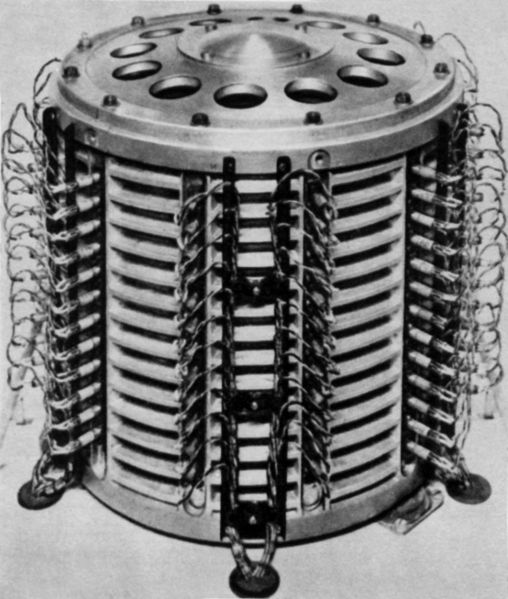
\includegraphics[width=0.3\linewidth]{memoire-images/tambour.jpg}
Dans les années 1970, cette technique était utilisée dans tous 
les ordinateurs\footnote{à l'exception de cas particuliers, comme 
les machines embarquées  et certains super-calculateurs}.

\subsection{Rappel : fonctionnement de la mémoire}

Différentes technologies ont été utilisées pour réaliser
les mémoires des ordinateurs : bascules bistables à base 
de tubes (triodes),
mémoires à tores de ferrite, à transistors,  
circuits intégrés etc.

\FIGURE{atlas-memoire-tores}{mémoire à tores de ferrite) ...}


Indépendamment des technologies, la mémoire est un organe
qui a pour fonction de stocker et restituer des ``mots binaires''
repérés par une \texttt{adresse}.

Les mots sont de taille fixe, par
exemple l'ATLAS avait une mémoire de 16384 mots de 48 bits. 
Les micro-processeurs
des années 75 étaient souvent des machines à octets (mot = 8 bits), de 
nos jours ce sont des mots de 32 ou 64 bits.

La mémoire communique avec le reste de l'ordinateur par
3 bus (groupes de fils)
\begin{itemize}
\item le \textbf{bus de contrôle} (il faudrait dire bus de commande), 
qui indique à la mémoire l'opération 
que l'on veut effectuer : 
\item le \textbf{bus de données}, bidirectionnel, qui sert à émettre et
recevoir les mots ;
\item le \textbf{bus d'adresses}, qui indique à la mémoire l'adresse
concernée.
\end{itemize}

\FIGURE{mod-initial.png}{La mémoire et ses trois bus}

\paragraph{Opérations :}
\begin{itemize}
\item \textbf{lecture} : pour consulter le contenu de la mémoire à
  l'adresse A, le processeur place le nombre A sur le bus d'adresses,
  et envoie le signal de contrôle ``lecture''. Après un petit délai de
  réponse, le contenu du mot d'adresse A est présenté par la mémoire
  sur le bus de données.
\item \textbf{écriture} : pour envoyer un mot M à l'adresse A, le
  processeur place A sur le bus d'adresses, M sur le bus de données et
  active l'ordre d'écriture.
\end{itemize}

%% \paragraph{Remarque :}  sur certaines machines (c'était le cas du 
%% processeur 8088 qui équipait
%% les premiers PC d'IBM\footnote{Le processeur 8086 d'INTEL possédait 
%% des bus séparés, le 8088 qui en était dérivé était à la fois plus cher
%% à fabriquer (c'est un 8086 avec en plus des circuits de 
%% multiplexage/démultiplexage) et moins performant. Ceci dit, le 8086 nécessitait une
%% famille de circuits associés 16 bits (contrôleurs d'interruption, etc), 
%% alors que le 8088 pouvait se contenter des circuits 8 bits qui étaient déjà produits
%%  en masse pour les microprocesseurs 8080 et 8085 qui équipaient les 
%%  micro-ordinateurs les plus courants de l'époque (sous CP/M).}), les bus de données et d'adresses 
%% sont \emph{multiplexés}, 
%% ils partagent des 
%% fils. L'avantage est de minimiser le nombre de connexions
%% entre circuits intégrés
%%  (et du nombre de pattes ), l'inconvénient est que les 
%%  données et les adresses ne sont  pas être transmis en même temps, 
%% ce qui se fait au détriment des performances.
%%  Un signal de commande supplémentaire précise si
%%  l'information qui circule est une adresse ou une donnée.

%% \subsection{Rappel : fonctionnement d'un processeur}

%% Un processeur est une machine électronique relativement simple, composée
%% de circuits logiques divers.  Il communique avec la mémoire (voir plus haut)
%% et les périphériques par des bus de données, d'adresse et de commande.

%% Son rôle est d'exécuter, les unes après les autres, des instructions
%% qui sont stockées en mémoire.

%% Un premier registre, appelé \textbf{compteur de programme}\footnote{ou pointeur 
%% d'instruction, compteur ordinal...} contient l'adresse de la prochaine
%% instruction à exécuter.  C'est un \emph{compteur} parce que, la plupart
%%  du temps, on va lui ajouter 1 pour passer à l'instruction suivante.

%% La première action du processeur est de lire en mémoire le mot qui contient cette
%% instruction, et de la placer dans un \textbf{registre d'instruction}, où il sera
%% décodé.

%% Par exemple, on aura peut être lu le mot de 32 bits
%% \textbf{000110000100001100000000000101010}
%% qui, sur un PowerPC 32 bits, se décompose en
%% \textbf{001110 00010 00011 00000000 000101010}
%% ce qui représente
%% \begin{itemize}
%% \item les 6 premiers bits : le code de l'opération ``ajouter une constante''
%% \item un numéro de registre destination (registre 2) sur 5 bits
%% \item un numéro de registre source (registre 3)
%% \item une constante (42) codée sur 16 bits
%% \end{itemize}
%% et qui signifie : ajoutez au registre de travail numéro 3 la valeur 42, 
%% et placez le résultat dans le registre 2, ce qu'on écrirait en 
%% \emph{langage 
%% d'assemblage} 
%% \begin{verbatim}
%% 	  addi  2,3,42
%% \end{verbatim}

%% L'exécution de l'opération ci-dessus fera appel à différents autres circuits
%% \begin{itemize}
%% \item les \textbf{registres généraux}, qui stockent des valeurs intermédiaires
%% (il y en a 32 sur le PowerPC)
%% \item une \textbf{unité arithmétique}, qui sera ici chargée de s'occuper de l'addition.
%% \end{itemize}

%% Certaines opérations permettront des transferts entre registres et mémoire, 
%% par exemple
%% \begin{verbatim}
%%    stw  5,0,1234
%% \end{verbatim}
%% envoie (store) le contenu du registre général 5 à l'adresse 1234 de la mémoire.

%% Il y a également des instructions pour comparer le contenu de registres,
%% et d'autres qui changent le cours de l'exécution si une condition
%% est remplie, en indiquant ne numéro de la prochaine instruction à exécuter.

%% En fait, les instructions de comparaison positionnent
%% des indicateurs booléens dans un \textbf{registre de condition}
%% qui mémorisent le résultat de la comparaison 
%% (inférieur, supérieur, égal ?)

%% En fonction de ces indicateurs, les \textbf{instructions de branchement 
%% conditionnel} incrémentent le compteur de programme, ou lui affectent 
%% une autre adresse.

%% \paragraph{Un exemple de programme en pseudo-assembleur}  vous permettra de voir
%% le niveau de détail auquel il faut descendre : la séquence ci dessous, 
%% qui commence à l'adresse 100, 
%% calcule la somme des entiers de 1 à N, en supposant que N est dans le registre 3
%% et que le résultat doit aller dans le registre 4. 
%% \begin{verbatim}
%% 100	   mettre la valeur 0 dans r4 
%% 101	   comparer r3 et la valeur 0
%% 102	   si égal, aller à 106
%% 103	   ajouter r3 à r4
%% 104	   ajouter la valeur -1 à r3
%% 105	   aller à 101
%% 106    ...
%% \end{verbatim}

%% Après l'exécution de l'instruction d'adresse 102, le compteur de programme
%% vaudra 103 ou 106, selon la valeur des indicateurs 
%% positionnés par l'instruction précédente (101).

%% Comme vous le voyez, un processeur n'est pas bien compliqué. C'est un assemblage 
%% de quelques circuits de base : registres, additionneurs, etc. qui sait exécuter
%% des instructions de base très élémentaires.

%% Ce qui est compliqué c'est de combiner des instructions 
%% aussi rudimentaires
%% pour effectuer des traitements utiles 
%% (qui ne sont pas forcément simples, eux). C'est la spécificité 
%% du travail du programmeur. 

\section{Adresses logiques et physiques}
\subsection{Le chargement des processus en mémoire}

Pour lancer un programme, un système d'exploitation multi-tâche
doit 
\begin{itemize}
\item réserver de la place en mémoire
\item y placer une copie de l'exécutable,
\item ajouter une entrée dans la table des processus, 
et la marquer comme prête.
\end{itemize}


Un même programme pourra donc être chargé à des endroits différents,
selon les programmes qui ont déjà été chargés.

Un nouveau problème se pose : un programme est composé d'instructions
élémentaires. Voici un exemple de programme écrit en \emph{langage
  d'assemblage} pour un processeur imaginaire.
\footnote{
\textbf{Description
  sommaire} : processeur très simple à un accumulateur. Les
  instructions contiennent l'adresse de l'opérande : pour
  charger/additionner/etc. une constante (zéro, un...) on utilise une
  variable contenant cette valeur. La comparaison \texttt{cmp}
  positionne des \emph{indicateurs} (inférieur, supérieur, égal) qui
sont utilisés par les instructions de branchement conditionnels 
(exemple : \texttt{bgt} = aller
à une adresse si plus grand - \emph{greater than}. L'instruction 
\texttt{b} est un branchement sans condition ; 
la directive \texttt{word} sert à réserver
un mot, avec une valeur initiale.
}
Exemple de programme:
\begin{lstlisting}[frame=single]
      load   zero
      store  somme
      load   un
boucle:
      store  i
      cmp    n    
      bgt    fin    ; sauter à fin si >  
      add    somme 
      store  somme
      load   i
      b      boucle ; aller à boucle
fin:
      halt
n     word   42
i     word   0
somme word   0
zero  word   0
un    word   1
\end{lstlisting}
Les instructions font référence à des adresses. En supposant que
chaque instruction tienne sur un mot, et que ce programme soit chargé
à l'adresse 100, l'instruction de saut ``b boucle'' fait référence à
l'adresse 103.

Si le codage de ``b boucle'' contient explicitement la constante 103, ce
programme ne fonctionnera pas correctement si il est chargé à une
autre adresse physique que 100.

\begin{exercice}
Faites tourner ce programme en fixant n à 4. Que fait-il, en général ?
\end{exercice}

Deux solutions ont été proposées pour ce problème 
\begin{enumerate}
\item au moment du chargement d'un programme, modifier les mots 
qui contiennent
des adresses pour tenir compte de début de la zone attribuée 
au processus.
\item différencier deux notions d'adresses : 
\begin{itemize}
\item l'\emph{adresse logique} : le début de la boucle est le
  cinquième mot du programme (adresse logique 4, puisque la
  numérotation commence à 0)
\item l'\emph{adresse physique} : ce mot se trouve dans la ``case''
  105 de mémoire.
\end{itemize}
\end{enumerate}

La première technique est faisable sans modification du processeur,
mais elle nécessite de garder une liste, à l'assemblage,
des emplacements qui contiennent des adresses, pour que le chargeur
puisse les modifier au chargement.

La seconde technique ne nécessite qu'une légère
modification du processeur, que nous allons détailler ci-dessous.


\subsection{Adresses logiques}

Avec les adresses logiques, tous les programmes sont compilés comme si
ils devaient être chargés à partir de l'adresse 0 de la mémoire.  Tout
se passe comme si chaque programme utilisateur s'exécutait dans une
mémoire qui lui appartient.


En réalité, les adresses logiques qu'il utilise sont traduites en
adresses physiques par un circuit MMU (\emph{memory management unit}) 
avant
d'être transmises à la mémoire : 
l'adresse logique est ajoutée au contenu d'un \textbf{registre de
base} contenant l'adresse de début de la zone mémoire allouée au
processus.

Cette modification ne  nécessite qu'un registre
et un additionneur.   

\FIGURE{mod-registre-base.png}{avec registre de base}

\subsection{Protection mémoire}

Quelques circuits supplémentaires fournissent une protection de
la mémoire : un \textbf{comparateur}\footnote{c'est un soustracteur où
  on ne regarde que le signe du résultat} vérifie que l'adresse
logique émise par le processeur est inférieure au contenu d'un
\textbf{registre limite}.

\FIGURE{mod-registre-base-et-limite.png}{avec registre limite}

Ceci garantit que le programme utilisateur reste confiné dans son
espace mémoire.

\subsection{Memory Management Unit}

À ce qui précède il convient d'ajouter qu'en mode privilégié le
processeur a normalement accès à toute la mémoire, avec des
instructions privilégiées qui lui permettent d'accèder explicitement
à des données  de l'espace utilisateur.

Par exemple, un appel système permet à un programme utilisateur de
demander l'écriture d'une chaîne de caractères, en précisant dans un
registre l'adresse de début du tableau de caractères.  Cet appel
système donne la main au système d'exploitation, qui doit interpréter
le contenu de ce registre comme une adresse dans l'espace utilisateur,
et non dans le sien.

On peut donc voir la MMU comme un circuit ayant
\begin{itemize}
\item \textbf{comme entrées :}
\begin{itemize}
\item une adresse logique AL
\item le contenu du registre de base RB,
\item le contenu du registre limite RL
\item un bit EU précisant l'espace d'adressage utilisé ( = 1 si 
utilisateur, ou instruction spéciale d'accès à l'espace 
utilisateur en mode privilégié)
\end{itemize}
\item \textbf{comme sorties :} 
\begin{itemize}
\item une adresse physique AP
\item un signal INT d'interruption si une violation mémoire s'est 
produite
\end{itemize}
\item les \textbf{équations logiques}  :

\begin{lstlisting}[frame=single]
     AP = si EU
            alors AL + RB
            sinon AL
     INT = EU et (AL >= RL)
\end{lstlisting}
\end{itemize}



\section{Gestion d'un espace mémoire linéaire}

Dans ce qui précède, chaque processus dispose d'un ``espace d'adressage
linéaire'' (ou plat) : l'ensemble des adresses logiques est une
séquence de nombres, sans trous ; et il lui correspond un ``bloc''
d'adresses contiguës en mémoire physique.


Dans un contexte de multiprogrammation, il va falloir gérer
l'allocation et la libération de ces blocs en mémoire, au fur
et à mesure que les programmes sont chargés et déchargés de la mémoire.

Pour simplifier l'explication, on se limite ici à un bloc par 
processus, mais
sur de nombreuses machines, le processeur comporte plusieurs paires de
registres base+limite, et les adresses logiques se réfèrent à l'un ou
l'autre des ``segments'' : segment de code, segment de données,
segment de pile, etc.\footnote{Ceci permet à la fois d'étendre les 
capacités
d'adressage en mode utilisateur (une adresse sur 16 bits donne
théoriquement accès à 64K mots dans un espace : avec 4 segments c'est
256K), et aussi de partager des segments entre plusieurs processus.
Par exemple, sur un système en temps partagé, on n'aura
en mémoire qu'un seul exemplaire du segment de code pour l'éditeur 
de textes,  
utilisé par des dizaines de personnes simultanément.} La problématique
sera la même : où charger les segments quand on en a besoin ?


\subsection{Exemple}

Supposons que nous disposions d'une mémoire centrale de 64K mots 
(confortable pour les années 60)

\FIGURE{dia-espace-memoire.png}{Espace mémoire de 64K mots}

et que nous souhaitions y charger 3 programmes de tailles respectives
10 K, 30 K et 15K. Une idée assez naturelle est de réserver un
espace mémoire consécutif pour chaque programme, et de placer
les programmes les uns à la suite des autres.

\FIGURE{dia-partage-memoire.png}{Placement consécutif}

Cette stratégie d'\textbf{allocation contiguë} parait simple, mais elle
pose un problème. A priori, on ne sait pas dans quel ordre les
 processus vont se terminer. Si c'est P1 qui se termine le
premier, la mémoire libre sera de 19K, mais il sera impossible de placer
un processus de 19K, puisque nous aurons deux blocs libres de 
10K (anciennement occupé par P1) et 9K, qui ne sont pas consécutifs.

Il faudra donc
\begin{itemize}
\item prendre des mesures si il se produit (déplacer les 
processus ?)
\item essayer d'éviter que ce problème ne se produise, du moins 
trop souvent,
\item ou alors remettre en cause l'idée de l'allocation contiguë.
\end{itemize}


%% \subsection{Adresses logiques}
%% \begin{itemize}
%% \item
%% \item
%% \end{itemize}

%% \subsubsection{Indépendance code/position physique}
%%  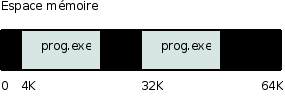
\includegraphics[width=0.9\linewidth]{memoire-images/indep-code-adr-physique.png}

%%  \FIGURE{indep-code-adr-logique.png}{Chaque processus a un espace d'adressage logique}
%%  Adresse physique =  adresse de base + adresse logique

%% \subsubsection{Modification du matériel}
%% registre de base

%% \FIGURE{mod-registre-base.png}{avec registre de base}
%% \FIGURE{reg8.jpg}{Registre 8 bits}
%% \FIGURE{add8.jpg}{Additionneur 8 bits}
%% \subsubsection{Protection inter-processus}
%% registre limite

%%  \FIGURE{core-war.png}{Jeu ``Core War'' (1984)}
%% \FIGURE{mod-registre-base.png}{(avec registre de base)}
%% \FIGURE{mod-registre-base-et-limite.png}{avec registre limite}
%% % \subsubsection{Résumé}

\subsection{Problème : la fragmentation}

%% \FIGURE{gruyere.jpg}{le gruyère n'a pas de trous}
%% \FIGURE{emmental.jpg}{confusion avec l'emmental}

Le scénario ci-dessous montre l'évolution de l'usage de la mémoire 
pendant qu'apparaissent et disparaissent des processus de tailles
diverses :
 
\FIGURE{frag-1.png}{(0) 3 processus sont présents, P2 se termine ...}
\FIGURE{frag-2.png}{(1) allocation de P4 ...}
\FIGURE{frag-3.png}{(2) allocation de P5 ...}
\FIGURE{frag-4.png}{(3) libération de P4 ...}
\FIGURE{frag-5.png}{(4) l'espace libre est fragmenté}


L'allocation et la libération de blocs de tailles diverses provoque
une \textbf{fragmentation} de l'espace mémoire disponible.  Cette
fragmentation peut rendre impossible le chargement en mémoire d'un
processus alors que l'espace libre total est en théorie suffisant.

\subsection{Solutions curatives}

Quand cette situation se produit, on peut envisager de décaler les
blocs alloués pour les ramener en début de mémoire, et ainsi regrouper 
toutes les zones libres en une seule. C'est possible si le processeur
distingue adresses logiques et adresses physiques ; le code des
programmes est alors ``relogeable'' (\emph{relocatable}) : il suffit
de le recopier ailleurs et de changer le contenu du registre de base.

L'inconvénient de cette opération de ``ménage'' est qu'elle oblige à 
interrompre les processus concernés pendant ce temps, provoquant des 
à-coups
désagréables dans un contexte d'utilisation interactive.

\begin{exercice}
Supposons qu'un ordinateur de 2Mo effectue un compactage toutes les 
secondes.
Si il faut $0.5 \mu s$ pour copier un octet, et si la taille moyenne
 des zones libres est égale à 0.4 fois celle des zones allouées, quelle
  fraction du temps du processeur est consacrée au compactage ?
\end{exercice}

\subsection{Solutions préventives}

L'exemple ci-dessus illustre la stratégie d'allocation dite
``\emph{first-fit}'' : les zones libres sont triées par ordre
d'adresses, et on choisit la première zone qui soit assez grande.  Une
partie de cette zone, correspondant à la demande, est allouée, et le
reste est replacé dans la liste des zones libres.

L'algorithme du \emph{meilleur ajustement} (\emph{best fit}) consiste
à retenir la plus petite zone qui soit assez grande. Son intention  est
d'éviter de fractionner les grands blocs.  Cependant les simulations
montrent qu'il fait perdre davantage de place que le ``best fit'' : en
effet il a tendance à créer de multiples petites zones libres, trop
petites pour être utilisables.

Inversement, l'algorithme du \emph{plus grand résidu} (\emph{worst
  fit}) choisit systématiquement le plus grand bloc libre.  En
pratique, ça ne donne pas non plus de bons résultats.

\begin{exercice}{Allocation contiguë}
La mémoire d'un système contient des zones libres de 10K, 4K, 20K,
18K, 7K, 9K, 12 K et 15K mots (dans l'ordre des adresses).
\begin{itemize}
\item Quelles zones l'algorithme \emph{first fit} choisit-il pour des
  demandes successives d'allocation de (a) 10K, (b) 12K, (c) 9K.
\item
Même question pour les deux autres algorithmes.
\end{itemize}
\end{exercice}

\subsection{Buddy system (blocs compagnons)}

Une autre approche : on évite de gérer des blocs de tailles trop
différentes. Pour cela on arrondit les demandes d'allocation mémoire à
la puissance de 2 supérieure (au dessus d'une valeur minimale
raisonnable, par exemple 1K octet).


Pour chaque taille , on maintient une liste de blocs : $L\_{10}$ 
(blocs de
$2^{10}=1024$ octets), $L_{11}$ (2048 octets), etc. qui commencent tous à
une adresse qui est un multiple de leur taille.  Par exemple les blocs
de $L_{11}$ peuvent commencer à l'adresse 0, 2K, 4K, 6K, etc.

\paragraph{Pour allouer} un espace de 3000 octets, la demande est 
arrondie à la puissance de 2 supérieure,
soit $2^{12} = 4096$.
 
On prend donc un bloc libre dans la liste $L_{12}$ des blocs libres de
4096 octets (si il n'y en a pas, on prendra dans la liste du dessus
$L_{13}$, etc.) commençant par exemple à l'adresse $12288 = 3 \times
2^{12}$.

L'excédent par rapport à la demande est de $4096-3000 = 1096$ : on
peut en retirer un bloc de 1024 octets qui est remis dans $L_{10}$. Le
bloc réellement alloué est de $4096 - 1024 = 3072$ octets.

\paragraph{Pour restituer} ce bloc de 3072 octets, il est fragmenté 
en un bloc de taille 
2048 ($2^{11}$) commençant à l'adresse $12288 = 3 \times 2^{12} = 6
\times 2^{11}$ qui est remis dans $L_{12}$, et un bloc de 1024
$2^{10}$ commençant en $12288 + 2048 = 3 \times 2^{12} + 2^{11} = 14
\times 2^{10}$ destiné à $L_{10}$.

Or ce dernier bloc est la moitié d'un bloc deux fois plus gros. Si
l'autre moitié (son bloc compagnon) - qui commence en $15 \times
2^{10}$) - est libre, on peut les fusionner en un bloc libre de
$2^{11}$ qui ira dans $L_{11}$.


Lors de la restitution, le bloc de 640 est à nouveau fragmenté en
$B_1$ (512) et $B_2$ (128). On consulte la liste L7 pour voir si le
{\em bloc compagnon $B'_2$} de $B_2$ y figure pas ($B_2$ est la moitié
d'un bloc de 256 octets, dont le compagnon est précisément l'autre
moitié).  Si il y est, on en profite pour fusionner les deux
compagnons pour faire un bloc libre de 256, dont on cherche le
compagnon dans L8, etc.

En pratique, ce système donne de bons résultats. 


\subsection{Partitions de taille fixe}

Une autre approche est l'utilisation de partitions de taille fixe.

Au démarrage, l'administrateur fixe un partage de la mémoire en
partitions. Dans une partition ne tournera qu'un programme qui lui
sera affecté soit explicitement, soit automatiquement (la plus petite
partition assez grande).

Le compactage est évité au prix d'une certaine perte de place.

Au début des années 80 le département de maths-info de Bordeaux 1
possédait un mini-ordinateur LSI 11-23 (Plessey), clone du PDP 11-23
de DEC, qui fonctionnait sous TSX-Plus. Avec ses 256 Ko de mémoire, il
permettait à 5 ou 6  utilisateurs de travailler en temps partagé
 depuis des
terminaux alphanumériques ou graphiques (Tektronix 4014 à écran
phosphore, très utilisé par les maths-applis, ou 4027 en couleur)
reliées par des lignes série.  Au démarrage, l'administrateur pouvait
fixer la taille de la partition mémoire allouée à chaque poste de
travail.


\section{Va-et-vient sur disque}

Dans un contexte d'utilisation en temps partagé conversationnel, on
s'aperçoit vite que l'utilisateur humain est de loin le périphérique
le plus lent du système.  Il lui arrive de lancer un programme (qui
prend de la place en mémoire) et de partir prendre un café (ou partir
en week-end) alors que le programme attend une réponse.

Dans ces conditions, on peut avoir l'idée de ``mettre de côté'' son
programme en faisant une copie sur disque de l'espace mémoire qu'il
utilise, espace qui sera bien bien plus utile si on le prête à des
programmes qui tournent vraiment.

\FIGURE{swapping-segment.png}{Échanges mémoire $\leftrightarrow$ disque}

Quand l'utilisateur reviendra et se décidera à appuyer sur une touche, 
le 
système ramènera le programme en mémoire, et poursuivra son exécution.

Dans la mesure où un accès disque ne prend que quelques centièmes de
seconde, le va-et-vient (swapping) du programme entre la mémoire vive
et le disque est imperceptible pour l'utilisateur interactif.

Économiquement, il faut aussi considérer le ratio des prix
entre mémoire centrale et disque : pour fixer les idées, début avril
2012, 1 Go de mémoire vive coûte environ 20 euros, et un disque de 1
To environ 100 euros, soit un rapport de 200.\footnote{
Ce rapport a évidemment beaucoup fluctué dans l'histoire de
l'informatique, mais il est clair qu'il revient moins cher de
``loger'' les processus inactifs sur disque qu'en mémoire vive. Et le
gain était d'autant plus clair à une époque où les sommes en jeu
n'étaient pas des dizaines d'euros, mais des dizaines de milliers de
dollars.}  

Le \emph{swapping} est donc une manière économique d'étendre la
capacité mémoire d'une machine, pour y faire tourner davantage de
programmes ``simultanément''.



\section{La mémoire segmentée}

Nous avons déjà vu l'idée de différencier adresses logiques et
physiques dans le cas d'un adressage ``plat'' (linéaire) : à chaque
processus correspond un ``bloc'' (ou segment) d'adresses contiguës de
la mémoire physique qui sont vues, par chaque processus utilisateur
comme un espace logique commençant à l'adresse 0.

L'astuce était d'employer un \emph{registre de base} qui indique
l'emplacement physique du premier mot de cette zone ; l'adresse
physique d'un mot s'obtient en ajoutant l'adresse logique au contenu
de ce registre.  Par exemple, si le registre de base contient 1734, le
mot d'adresse logique 55 est situé à l'emplacement $1734+55=1789$ de
la mémoire physique.

\subsection{Segments}

Le besoin est vite apparu de permettre au processeur d'accéder à
plusieurs segments.  Par exemple, dans un usage interactif, il se peut
que plusieurs utilisateurs fassent tourner le même programme.  Dans ce
cas, il serait dommage de charger autant d'exemplaires du code
exécutable que d'utilisateurs ; il est plus judicieux de considérer
que l'espace mémoire d'un programme se compose de deux segments : 
\begin{itemize}
\item le
segment de code contenant les instructions (qui peut être partagé),
\item et le segment de données où se trouvent les variables propres à
chaque instance du programme.
\end{itemize}
\FIGURE{seg1.png}{Deux processus exécutent le même code}

Plus généralement, les programmes présents en mémoire, même si ils
sont différents, font souvent appel à des bibliothèques
(\emph{libraries}), par exemple les fonctions mathématiques.
Chaque bibliothèque peut être chargée en mémoire comme un segment
de code qui sera éventuellement partagé.

Ce besoin est apparu très rapidement : la première machine
commerciale à utiliser la segmentation est le B5000 de Burroughs,
 sorti en
1961.

\subsection{Espace d'adressage}

On s'éloigne donc de l'adressage plat, où les adresses logiques d'un
processus sont dans un intervalle $[0..n]$. Dans une mémoire segmentée,
les adresses sont maintenant
formées d'un couple (s,p) avec
\begin{itemize}
\item un numéro de segment \texttt{s} 
\item une position \texttt{p} dans le segment (on parle
  d'\emph{offset}, ou de déplacement)
\end{itemize}
Le numéro de segment est toujours placé dans les bits de poids forts
de l'adresse.


\paragraph{Exemple, le PDP  10} utilisait des adresses de 18 bits
 comportant 
\begin{itemize}
\item un bit pour le numéro de segment
\item 17 bits pour la position dans le segment
\end{itemize}
ce qui veut dire que l'espace mémoire logique se décomposait en 2
segments, et que le processeur comportait deux registres de base (et
deux registres limite).


\begin{tabular}{|c||c|ccccc|}
\hline
numéro de bit & 17 &16 &15& ... & 1 &0 \\
\hline
& s & p & p & .. & p & p \\
\hline
\end{tabular}

d'au plus $2^{17}$ = 128 K mots chacun. Les adresses du ``segment
bas'' commencent à 0 à 128K-1, celles du ``segment haut'' à partir de
128K.  L'espace d'adressage n'est plus linéaire : si le processus a un
segment bas de 4K et un segment haut de 8K, les adresses logiques
valides sont dans deux plages séparées : de 0 à 4K-1 et de 128K à
136K-1.

Selon la valeur du bit 17, on sélectionne l'un ou l'autre des 
registres de base

\FIGURE{impl1.png}{un multiplexeur sélectionne le registre de
 base à utiliser}

\begin{exercice}
Soit une machine dont les adresses, sur 24 bits, comportent 4 bits
pour le numéro de segment.
\begin{enumerate}
\item combien y a t-il de segments logiques ?
\item quelle est la taille maximum d'un segment ?
\item quelle est la taille de l'espace d'adressage logique ?
\item quelle est l'adresse logique correspondant à l'octet 2 
du segment 5 ?
\item donnez le numéro de segment et l'offset de l'adresse 
logique 0x600042.
\end{enumerate}
\end{exercice}

\subsection{La réalisation}

Prenons le cas d'une machine dont les adresses sur 20 bits, (notées
\texttt{AL[19:0]}) comportent 2 bits pour le numéro de segment
\texttt{AL[19:18]} et 18 bits \texttt{AL[17:0]} pour le déplacement.

Cette machine a donc une table de segments composée de 4 registres de
base \texttt{RB[i]} et autant de registres limites \texttt{ RL[i]}.

L'adresse logique se calcule donc en additionnant
\begin{itemize}
\item le contenu du registre correspondant au numéro de segment
\item  le déplacement contenu en partie basse de l'adresse
\end{itemize}
\begin{lstlisting}
AL =  RB[  AL[19:18] ] +  AL[17:0]
\end{lstlisting}

\FIGURE{impl2.png}{utilisation d'une table des segments}

et une violation de protection mémoire est détectée si le déplacement
atteint ou excède la limite du segment.
\begin{lstlisting}
INT = 1 si  AL[17:0] >=  RL[ AL[19:18] ]
      0 sinon
\end{lstlisting}

\paragraph{La taille des registres limite} est logiquement, 
sur cet exemple,
de 18 bits, puisqu'ils servent à vérifier un déplacement qui est lui-même
exprimé sur 18 bits.  Par contre on se sait rien sur la taille des
registres de base. En effet, si l'espace adressable par un processus
est limitée à $2^{20} = $ 1M mots à travers 4 segments de 256K mots, la
mémoire physique peut être plus grande pour accueillir plusieurs
processus. Par exemple, on peut avoir des adresses physiques sur 24
bits, ce qui donne une capacité de 16M mots pour la mémoire physique.

\begin{exercice}
Le processeur 8086 utilisait 4 registres de base CS, SS, DS et
ES\footnote{segments de code, de pile, de données et supplémentaire},
des déplacements sur 16 bits, et des adresses physiques sur 20
bits. Les segments commençaient à des adresses multiples de 16, les
registres de base contenaient les 16 bits de poids fort qui étaient
virtuellement complétées par 4 zéros binaires.
\begin{enumerate}
\item quelle est la capacité maximum de la mémoire physique ?
\item quelle est la taille de l'espace d'adressage d'un programme à un
  moment donné ?\footnote{les programmes pouvant modifier leurs
    registres de base, ils ont accès à tout}
\item si CS contient 0x5432, quelle est l'adresse physique
  correspondant à l'adresse 0x0123 du segment de code ?
\end{enumerate}
\end{exercice}

\subsection{Tables locale/globale des segments}

En réalité c'est un petit peu plus compliqué. Si un programme a été
compilé pour utiliser 3 segments - par exemple 0 = le code, 
1 = les données 
et 2 = la
bibliothèque mathématique -, la numérotation utilisée pour les segments
est \textbf{locale} au processus : la bibliothèque mathématique peut
être le segment 2 de ce processus, et le segment 4 d'un autre.

Par contre, les informations sur les segments (position en mémoire,
taille, attributs de protection,...)  sont \textbf{globales} à tout le
système.

On utilise donc deux tables
\begin{itemize}
\item la \textbf{table globale des segments} (TGS), qui garde trace de
  tous les segments chargés en mémoire
\item une \textbf{table locale des segments} (TLS) pour le processus
  en cours, dans laquelle se fait la correspondance entre le numéro de
  segment utilisé dans les adresses logiques, et le numéro global de
  segment
\end{itemize}

La traduction d'une adresse logique (s,d) passe donc par
\begin{itemize}
\item la consultation de TLS[s] pour trouver le numéro g de segment
  global correspondant à s. Par exemple on trouvera que le segment
  local 2 est le segment global numéro 17.
\item la consultation de la TGS[g] pour récupérer l'adresse de base et
  la taille du segment. Par exemple le segment global 17 commence en
  0x12345678.
\item l'addition de l'adresse de base au déplacement pour obtenir
  l'adresse physique. L'adresse 12 du segment 2 est donc en
  0x1234568A.
\end{itemize}

\FIGURE{generation-segmentation.png}{Génération d'adresses, TLS + TGS}

La table globale des segments contient des
\textbf{descripteurs}, qui indiquent pour chaque segment
\begin{itemize}
\item la position du segment en mémoire
\item sa longueur
\item les droits d'accès (lecture, écriture, exécution)
\end{itemize}

En effet il est assez simple, au niveau du processeur d'émettre des
signaux qui indiquent son état (recherche d'une instruction,
exécution, ...)  La MMU peut donc vérifier que le processeur n'essaie
pas d'exécuter des instructions dans un segment qui est censé ne
contenir que des données, ce qui correspond à une lecture en mémoire
pendant la phase d'exécution sur un segment non-exécutable.

C'est très utile notamment pour lutter contre les attaques par
``débordement de buffer''. Dans une telle attaque, un utilisateur
malveillant envoie des données d'une taille supérieure à celle de la
variable tampon destinée à les recevoir\footnote{Il y a là une faute
  du programmeur qui n'a pas contrôlé la taille des données reçues
  avant de les placer dans le tampon}. En effet, cette variable tampon
se trouve sur la pile d'exécution, où se trouve également l'adresse à
laquelle la fonction devra retourner.

En choisissant soigneusement les données envoyées, le pirate s'arrange
pour charger du code en mémoire, et remplacer l'adresse de retour de
la fonction pour qu'elle désigne ce code. Quand la fonction fera son
``return'', c'est le ``code malicieux'' qui sera exécuté.

Voir article ``dépassement de tampon'' sur Wikipédia.


% 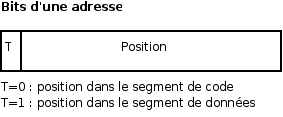
\includegraphics[width=0.9\linewidth]{memoire-images/format1.png}


\subsection{Espace mémoire paginé}

Revenons au problème qui se posait pour la gestion de la mémoire,
inhérent au fait de gérer des segments de tailles diverses, qui
apparaissent et disparaissent au cours de l'évolution du système, en
laissant des trous inexploitables.

Une solution a été trouvée, là encore très tôt dans l'histoire de
l'informatique : considérer chaque segment non comme un espace
linéaire, mais comme une suite de \emph{pages}, qui ne sont pas
forcément placées séquentiellement en mémoire.

\FIGURE{pagination.png}{espace paginé}

À la différence des segments, les pages sont de même taille, qui est
une puissance de 2 (valeurs courantes = 1, 2, 4, 16K), et elles sont
alignées sur un multiple de la taille de page. En supposant des pages
de 4K, la page 0 est en 0, la page 1 en 4K, la page 2 en 8K, etc.


Considérons par exemple une machine dont les adresses logiques sont
sur 16 bits (espace d'adressage de 64 Kmots), avec des pages de 4K
mots. La position d'un mot dans une page sera donc un nombre compris
entre 0 et 4K-1, qui sera exprimé sur 12 bits (puisque $2^{12} =
4K$). 

Une adresse logique se composera donc
\begin{itemize}
\item de $16-12=4$ bits pour le numéro de page, qui sera compris entre
  0 et $15=2^{4}-1$ ;
\item de 12 bits pour le déplacement dans la page.
\end{itemize}

\FIGURE{format-pagination.png}{format d'adresse logique}

On a vu que la mémoire physique peut être de taille différente, par
exemple 256K mots, et comporte donc $\frac{256K}{4K} = 64$
\textbf{cadres de page}\footnote{on parle de pages pour l'espace
logique, et de cadres de pages pour l'espace physique}

\begin{exercice}
\begin{itemize}
\item quelle est la taille d'une adresse physique ?
\item combien de bits dans un numéro de cadre de page ?
\end{itemize}
\end{exercice}

La \textbf{table des pages} indique où se trouvent
les cadres de page en mémoire

\begin{tabular}{|c||cccccccc|}
\hline
page & 0 & 1 & 2& 3 & 4 & 5 &6 & 7 \\
cadre & 6 & 7 & 23 & 1 & 42 & 17 & 18 & 62 \\
\hline
\end{tabular}


Quand un processus s'exécute, sa table des pages est chargée dans les registres
de page de la MMU, qui effectue la traduction.

L'adresse physique est formée en concaténant 
\begin{itemize}
\item le contenu du registre correspondant
au numéro de page (en poids forts de l'adresse logique) 
\item la position dans la page (bits de poids faibles de l'adresse logique)
\end{itemize}

\begin{lstlisting}
AP[17:12] =  RP[  AP[15:12]  ]
AP[11: 0] =  AL[11:0]
\end{lstlisting}

\FIGURE{generation-pagination.png}{génération d'adresse}

\begin{exercice}
Déterminer les adresses physiques correspondant aux adresses logiques
\texttt{0x00F0}, \texttt{0x32AB}, \texttt{0x1030}. 
\end{exercice}

%% \FIGURE{oeuf-colomb.jpg}{}

\subsection{Un circuit MMU : le MC68851}
 
Le MC68851, un des premiers circuits MMU pour microprocesseurs, était
destiné à compléter le microprocesseur 68020 qui équipait notamment
les MacIntosh II et LC, les Amiga 1200 et la console CD32, les
stations graphiques IRIS et Sun-3.

 Vous pouvez trouver sa ``datasheet'' 
sur internet : \url{ http://pdf1.alldatasheet.com/datasheet-pdf/view/4166/MOTOROLA/MC68851.html}

Voici quelques-unes de ses fonctionnalités
\begin{itemize}
\item Full 32-bit logical to physical address ;
\item Wide selection of page size from 256 Bytes to 32 KBytes ;
\item fully associative, 64-entry, on chip address translation cache ;
\item automatic update of the onc-chip translation cache from external translation tables ;
\item multiple tasks supported simultaneously ;
\end{itemize}
que nous allons examiner, et qui permettront de mieux comprendre comment
fonctionne un vrai circuit MMU.

\paragraph{Adresses logiques et physiques sur 32 bits : } la MMU s'intercale entre le processeur et la mémoire. Les bus d'adresses peuvent en principe être de taille différentes, ici ce sont les mêmes. À quoi cela sert-il ?
\begin{itemize}
\item il faut d'abord penser qu'en 1984 (année de sortie du 68020),
  les machines auxquelles ce processeur était destiné disposaient au
  mieux de quelques méga-octets de mémoire.
\item cependant, rien n'empêche un programmeur d'utiliser la plage
  d'adresses logiques à sa guise. Sur un système paginé on peut simuler la
  segmentation en utilisant par exemple les 8 bits de poids forts comme numéros de
  segments. Cela n'impliquera pas que le segment 0xFF commence physiquement
à l'adresse 0xFF000000, ni que la machine dispose de 4 G ($2^{32}$)
  octets de mémoire réelle.
\item une des rôles de la MMU est donc de ``mapper'' les adresses
  logiques utilisées (espace logique qui comporte beaucoup de trous)
  sur la plage d'adresses physiques qui est bien plus petite.
\end{itemize}

\paragraph{Taille de pages de 256 à 32 K octets : } selon le type 
d'utilisation on pourra avoir intérêt à avoir des petites pages ou des
grandes pages, et le circuit était configurable pour correspondre aux besoins.
\begin{itemize}
\item pendant l'allocation mémoire, la taille demandée est arrondi au
  multiple suivant de la taille des page. Par exemple, pour 20K octets
  on utilisera 80 pages de 256 octets, ou 1 page de 32K. Dans ce
  dernier cas, on gaspille 12 Ko.  En moyenne, le gaspillage est d'une
  demi-page.
\begin{exercice}  Un des arguments contre la pagination (opposée à la mémoire partitionnée)
était que ça faisait perdre une place non négligeable en
mémoire. C'est à relativiser selon la taille de la mémoire, des programmes, etc. Comparez les pourcentages de perte dans
ces situations :
\begin{itemize}
\item une machine des années 60, avec 64Ko de mémoire (pages de 4Ko)
  qui fait tourner des programmes de quelques kilo-octets
\item un PC actuel (pages de 4K à 2M) utilisé comme serveur
\item un PC domestique
\end{itemize}
et tirez une conclusion, dans chaque contexte d'utilisation.
\end{exercice}


\paragraph{Support simultané de taches multiples} : lors d'un
changement de contexte, le processeur indique à la MMU un numéro de
tâche sur 3 bits. Les adresses logiques qui suivront seront alors interprétées par 
rapport à l'espace logique de cette tâche.


\paragraph{Table associative} à 64 entrées pour la 
génération d'adresses, mise à jour automatiquement depuis des tables
en mémoire : 
\begin{itemize}
\item la MMU ne contient pas toute la table des pages, mais seulement
  64 éléments qui contiennent chacun un numéro de page logique
  (combiné au numéro de tâche) et le numéro de la page physique. Le
  reste de la table réside dans la mémoire physique.
\item lorsque le système d'exploitation effectue un changement de tâche,
il indique à la MMU l'adresse de la ``racine'' de la table des pages de la tâche.
La MMU garde une racine pour chaque tâche.
\item lors d'une traduction d'adresse, le numéro de page logique
  (combiné avec le numéro de tâche) est comparé aux 64 numéros de
  pages logiques présents dans le ``cache'' de la MMU.\footnote{C'est
    une comparaison \textbf{simultanée} grâce à 64 circuits
    comparateurs qui travaillent en parallèle, un par registre. C'est
    ce qu'on appelle une mémoire associative}

Si le numéro de page logique est absent du cache, la MMU va
  chercher le numéro de page dans la table en mémoire, pour remplacer
  le contenu du registre utilisé le moins récemment.

\end{itemize}
\end{itemize}




\section{Mémoire virtuelle paginée}

\subsection{Principe}

La pagination permet apporte une grosse amélioration de la technique
de va-et-vient sur disque exposée plus haut.  En effet, pour relancer
un programme qui a été ``swappé'' sur le disque, il suffit de
recharger depuis le disque la page qu'il était en train d'exécuter, et
non l'intégralité de son espace mémoire.



L'espace d'échange sur disque, qui est lui-même structuré en ``pages''
de même taille.  L'ensemble, mémoire vive + espace d'échange,
constitue une mémoire virtuelle qui peut être beaucoup plus grande que
la seule mémoire vive.


\FIGURE{swapping.png}{Swapping}

On constate par ailleurs que, pendant l'exécution d'un programme,
celui-ci ne fait référence qu'à quelques pages à la fois. Il est assez
probable qu'après avoir exécuté l'instruction N, il passe à
l'instruction N+1, où à une autre instruction proche : en pratique la
plupart des boucles et de sauts ne vont pas très loin, le plus souvent
la destination est dans dans la même page.

Automatiquement, les pages qui ont été transférées sur disque y
restent tant qu'on n'en a pas besoin, et libèrent autant de place pour
les pages les plus ``actives'' des processus, on fera donc une
économie de place, qui permettra d'avoir davantage de processus
``présents'' (processus prêts, avec leur page active déjà présente en
mémoire vive).  D'où de meilleures performances qui si on chargeait en
totalité l'espace mémoire d'un processus.

\subsection{MMU pour la mémoire virtuelle paginée}

Une page peut être présente en mémoire ou non, et si elle ne l'est
pas, elle peut être sur le disque.  La table des pages indique donc le
numéro de cadre de page, et le numéro de bloc dans l'espace disque
réservé au swap.

La table des pages pour la mémoire paginée comporte donc ces informations

\begin{tabular}{|c|cccc|}
\hline
page logique  & 0 & 1 & 2 &..... \\
\hline
cadre (physique) &  17 & - & 3 & .... \\
sur disque  & 42 & 13 & 44 & ... \\
\hline
\end{tabular}

La MMU contiendra, comme précédemment, une table de registres pour la
correspondance entre numéro de page et numéro de cadre, et des
indicateurs de présence pour les pages.  Une interruption de ``défaut
de page''\footnote{qui signifie que la page fait défaut (elle manque),
  et non pas qu'elle est défectueuse} sera émise si un accès est tenté
à une page absente.

Exemple :

\begin{lstlisting}
DEFAUT_DE_PAGE = non PRESENT[  AP[15:12]  ]
AP[17:12] =  RP[  AP[15:12]  ]
AP[11: 0] =  AL[11:0]
\end{lstlisting}

L'interruption provoquera l'intervention du système d'exploitation qui
\begin{enumerate}
\item consultera la table des pages pour trouver l'emplacement, sur
  disque, de la page manquante
\item trouvera un cadre de page libre en mémoire. 
\item procédera au chargement de la page en mémoire
\item mettra à jour la table des pages
\item relancera le processus interrompu
\end{enumerate}

Pour trouver un cadre de page, il faudra souvent (dès que la mémoire
réelle sera pleine) faire de la place en transférant sur disque une
page présente. La manoeuvre de remplacement comportera donc deux accès
disque, l'un pour sauver sur disque la page qui est en mémoire,
l'autre pour lire sur disque la page à ramener en mémoire.

Deux accès disques représentent dans le meilleur des cas quelques
centièmes de seconde, ce qui est très long à l'échelle de
l'ordinateur. On cherchera donc à minimiser le nombre de  défauts de page.


 
\subsection{Les algorithmes de remplacement de page}

Dans le cadre de ce mécanisme très général il reste à définir la
méthode pour choisir (second point) le cadre de page dans lequel la
page manquante va être amenée en mémoire. C'est l'objet des
\textbf{algorithmes de remplacement de page}.

En réalité ce sont plus des heuristiques que des algorithmes : un bon
algorithme devrait trouver une solution optimale, or c'est impossible
dans l'absolu : à un moment donné on décide de remplacer telle page
plutôt qu'une autre, c'est seulement dans le futur, selon la suite des
évènements, que cette décision apparaîtra
judicieuse ou non.

Or le futur est, en grande partie, imprévisible. On utilisera donc des
\textbf{heuristiques}, méthodes dont l'objectif est d'obtenir des
résultats acceptables dans la plupart des cas.


\subsection{Remplacement à tour de rôle}

Le premier algorithme, appelé aussi FIFO (first-in first out, premier
entré premier sorti) consiste à utiliser à tour de rôle chacun des
cadres de pages. C'est une méthode simpliste, qui ne donne pas de bons
résultats (nous verrons pourquoi), que nous exposons surtout pour
introduire quelques idées.

L'exécution d'un programme provoque de nombreux accès successifs à la
mémoire. Ces adresses correspondent à des pages, dont nous retiendrons
les numéros, qui constituent la \emph{séquence de références de
  pages}.  Par exemple un processus fera accès aux pages
22,33,22,17,44,18,22,12,33,22,...

Pour simplifier l'explication, prenons un mémoire physique de 4 cadres
de pages seulement.\footnote{ce qui est très éloigné des ordres de
  grandeurs réels : un mini-ordinateur typique des années 80, avec quelques
  mega-octets de mémoire, a des centaines ou des milliers de cadres de page.}

Un tableau nous servira à montrer quelle page occupe quel cadre, au
fur et à mesure du déroulement de la séquence d'accès :


%% { \tiny
%% \begin{tabular}{|c|cccccccccc|}
%% \hline
%% temps &1 & 2 & 3 & 4 & 5 & 6 & 7 & 8 & 9 & 10 \\
%% page & 22 & 33 & 22 & 17 & 44 & 18 & 22 & 12 & 33 & 22 \\
%% \hline
%% cadre 1 & & & & & & & & & &  \\
%% cadre 2 & & & & & & & & & & \\
%% cadre 3 & & & & & & & & &  & \\
%% cadre 4 & & & & & & & &  & & \\
%% \hline
%% \end{tabular}
%%}

Après quelques étapes, le tableau est ainsi rempli

\begin{center}
 { 
\tiny
\begin{tabular}{|c|cccccccccc|}
\hline
temps &1 & 2 & 3 & 4 & 5 & 6 & 7 & 8 & 9 & 10 \\
page & 22 & 33 & 22 & 17 & 44 & 18 & 22 & 12 & 33 & 22 \\
\hline
cadre 1 & \fbox{22} & 22 & 22 & 22 & 22 & \fbox{18} & 18 & & &  \\
cadre 2 & - & \fbox{33} & 33 & 33 & 33 & 33 & \fbox{22}& & & \\
cadre 3 & - & - & -  & \fbox{17}& 17 & 17 & 17& &  & \\
cadre 4 & - & - & - & - & \fbox{44} & 44 & 44 &  & & \\
\hline
\end{tabular}
}
\end{center}

\begin{itemize}
\item au début tous les cadres de  pages sont vides
\item aux temps 1,2,4 et 5 les cadres de pages sont chargés
  successivement avec les pages demandés (les défauts de page sont
  encadrés).
\item remarquez qu'au temps 3 la page demandée est déjà présente, il
  n'y a donc pas d'accès au disque.
\item à t=6 tous les cadres de pages sont occupés. L'algorithme
  choisit de charger la page manquante dans le cadre 1.
\item même problème ensuite : on passe au cadre 2
\end{itemize}

\begin{exercice}
\begin{itemize}
\item Complétez le tableau.
\item Combien de défauts de page ?
\end{itemize}
\end{exercice}

\begin{exercice} On appelle \textbf{oracle} un algorithme (hypothétique) qui serait capable de prendre les meilleures
décisions en tenant compte de l'avenir. Que ferait un oracle dans ce
cas ?
\end{exercice}

\paragraph{Anomalie de Belady}.  Il est raisonnable de penser
que plus on dispose de mémoire, moins on aura de défauts de
page. 

Dans les années 60 on pensait que c'était une règle générale, mais en
1969 Laszlo Belady a trouvé un contre-exemple\footnote{probablement en
essayant de démontrer que c'était vrai} :

\begin{exercice}
Soit la  séquence de références 1 2 3 4 1 2 5 1 2 3 4 5 
\begin{itemize}
\item calculez le nombre de défauts de page obtenus avec l'algorithme FIFO
pour 3 cadres de pages
\item même question pour 4 cadres de pages
\end{itemize}
\end{exercice}

C'est un exemple de ``scénario pathologique'' qui montre qu'une
affirmation généralement acceptée (``il vaut mieux être riche et en
bonne santé que pauvre et malade'') n'est pas vraie dans \emph{tous}
les cas.  Cependant l'existence de contre-exemples n'empêche pas
l'affirmation d'être vraie presque tout le temps.

\paragraph{Note.} On a longtemps estimé que les séquences pathologiques
produisaient au maximum deux fois plus de défauts de page. Deux chercheurs
ont montré en 2010 (\url{http://arxiv.org/abs/1003.1336}) que le ratio
des nombres de défauts de page n'est pas borné.


\subsection{Algorithme LRU : least recently used}

L'algorithme FIFO ci dessus ne donne pas de bons résultats en
pratique, parce qu'il ne tient pas compte d'une propriété importante
du comportement des programmes, la \textbf{localité}. 

\paragraph{Principe de localité} : pendant le déroulement d'un vrai programme, il est très probable
qu'après avoir exécuté une instruction, la suivante soit très proche,
presque certainement dans la même page.  Et qu'après avoir accédé à un
élément de tableau, on passe au suivant.

Cette propriété de localité fait que si un programme a besoin
d'accéder à une page, c'est très probablement une des pages qu'il a
utilisées il y a peu de temps.

On met à profit ce principe, en conservant les pages qui ont été
utilisées le plus récemment. L'algorithme qui en découle consiste donc
à choisir le cadre qui contient \textbf{la page accédée le moins
  récemment}, d'où son nom (LRU = least recently used).

Le tableau ci-dessous montre le déroulement de l'algorithme LRU. 

\begin{center}
 { 
\tiny
\begin{tabular}{|c|cccccccccc|}
\hline
temps &1 & 2 & 3 & 4 & 5 & 6 & 7 & 8 & 9 & 10 \\
page & 22 & 33 & 22 & 17 & 44 & 18 & 22 & 12 & 33 & 22 \\
\hline
cadre 1 & \fbox{\textbf{22}} & 22 & \textbf{22} & 22 & 22 & 22 & \textbf{22} & & &  \\
cadre 2 & - & \fbox{\textbf{33}} & 33 & 33 & 33 & \fbox{\textbf{18}}& 18 & & & \\
cadre 3 & - & - & -  & \fbox{\textbf{17}}& 17 & 17 & 17& &  & \\
cadre 4 & - & - & - & - & \fbox{\textbf{44}} & 44 & 44 &  & & \\
\hline
\end{tabular}
}
\end{center}

\begin{itemize}
\item Les caractères gras marquent les accès.
\item à t=6, on choisit le cadre 2 pour lequel le dernier accès a eu
  lieu à t=2, contre 3,4 et 5 pour les autres.
\end{itemize}


\begin{exercice}
\begin{itemize}
\item Complétez le tableau.
\item Combien y a t'il de défauts de page ?
\end{itemize}
\end{exercice}




\paragraph{Réalisation matérielle}

Pour pouvoir appliquer cet algorithme il faut ajouter un peu de
matériel dans la MMU : pour chaque page un \emph{estampille}, registre
qui contiendra la date de dernier accès (\emph{horodatage}). Cette estampille sera mise à jour à chaque accès en y
copiant la valeur d'un compteur qui s'incrémente sous le contrôle
d'une horloge.

Le système d'exploitation interrogera la MMU pour relever les compteurs quand 
un défaut de page se produira.

\begin{exercice}
En théorie ce compteur, mis à zéro au démarrage, devrait être
incrémenté à chaque instruction. De quelle taille devrait-il être pour
une machine qui exécute 1 million d'instructions par seconde, et qui
fonctionne sans arrêt pendant une année ?
% 31.5 millions de secondes dans une année soit à peu près 32 x 10^12 instructions.
% 10^3 = à peu près 2^12, donc  32 x 10^12 = 2^51 ?
\end{exercice}

En pratique, les transistors coûtent cher sur une MMU, et on se
contentera d'une précision moindre, en ne stockant que les bits de
poids fort du compteur.  Nous verrons plus loin l'algorithme NRU (not
recently used), dans lequel on se contente d'un bit pour différencier
les pages récemment accédées de celles qui ne le sont pas.

\paragraph{Scénarios pathologiques} : en général
les algorithmes basés sur la localité marchent bien en pratique, parce
que c'est un comportement qu'on observe sur les vrais programmes.
Cependant il est tout-à-fait possible de construire des
contre-exemples.

\begin{exercice} Soit l'affirmation ``le LRU fait moins de défauts de page que que FIFO''.
Considérons un système avec 3 cadres de pages. La séquence de
références de pages commmence par 11, 22, 33. Si on la prolonge par 11
et 44, l'algorithme FIFO placera la page 44 dans le cadre 1, et LRU
dans le cadre 2.
\begin{itemize}
\item 
À partir de là, les situations ayant divergé, continuez la séquence
avec des numéros bien choisis pour que la stratégie LRU conduise à
plus de défauts de page que FIFO.
\item Votre conclusion ?
\end{itemize}
\end{exercice}

Attention : l'existence de contre-exemples ne prouve pas que LRU n'est
pas meilleur que FIF0, seulement qu'il peut exister des cas
pathologiques où ça se passe moins bien que ce qu'on pensait. Or ces
cas, précisément, sont construits en ignorant le principe de localité,
et en raisonnant sur un nombre totalement irréaliste de cadres de
pages\footnote{Un petit programme pour PC occupe quelques mégas
  octets, soit des milliers de pages. La probabilité d'apparition d'un
  scénario pathologique est assez faible.} On est donc loin de la
``réalité statistique''.


\subsection{NRU, remplacement d'une page non récemment utilisée}

Deux bits sont associés à chaque page : R  indique si la page a été
{\em référencée} (en lecture ou en écriture), M qu'elle a été modifiée.
Ces deux bits sont positionnés à chaque référence mémoire.

Périodiquement, le système remet les bits R des pages à 0.  Si le bit
R d'une page est à 1, on peut donc en conclure que la page a été
référencée récemment.

On obtient donc 4 catégories de pages :
\begin{enumerate}
\item pages non référencées, non modifiées (R=0, M=0),
\item pages non référencées, modifiées (R=0, M=1),
\item pages référencées, non modifiées (R=1,M=0),
\item pages référencées et modifiées (R=1, M=1).
\end{enumerate}

L'algorithme NRU ({\em not recently used}) choisit au hasard une des
pages de la  première catégorie non vide.

En pratique cet algorithme est facile à implémenter, relativement efficace,
et ses performances sont généralement suffisantes.



\subsection{Algorithme de la seconde chance}

Variante de l'algorithme FIFO, en utilisant le bit R. Lors d'un défaut
de page, l'algorithme teste le bit R de la page la plus ancienne. Si
il est à 1, la page est remise en fin de liste avec son bit R mis à 0
(comme si elle venait d'être chargée), et l'algorithme regarde la page
suivante, jusqu'à trouver une page ayant le bit R à 0, qui sera
retirée.

En pratique on utilise une liste circulaire. Exercice : justifier
son autre appellation : {\em algorithme de l'horloge}.


\subsection{Algorithme du vieillissement}

On utilise le bit de référence R, et un registre à décalage 
vers la droite de n bits pour chaque page.
À intervalles réguliers, le bit R est transféré dans le registre
à décalage, puis remis à 0.

Le registre à décalage permet donc de savoir si des références ont
été faites lors des n dernières périodes de temps. Par approximation
grossière, un grand nombre dans le registre (beaucoup de bits 1 à gauche)
indique qu'une page a été récemment beaucoup utilisée.


\subsection{Réservation d'espace d'échange}

On peut se poser la question : où vont les pages évacuées ? 
Leur a-t-on préalablement réservé un espace sur le disque, ou non ?


La réponse dépend de la philosophie adoptée pour la mémoire
virtuelle. L'ancienne école considérait que les processus
``habitaient'' dans l'espace disque réservé pour le swapping, et
qu'ils ne faisaient que passer provisoirement dans la mémoire vive,
considérée comme un {\em cache} du disque dur.  Dès son lancement, un
processus se voyait donc réserver une place dans l'espace de swap, qui
devait être au moins aussi grand que la mémoire vive.

On peut aussi considérer que l'espace de swap est une extension de la
mémoire.  Un processus est chargé en mémoire sans se préoccuper de
réserver de l'espace sur disque. Il pourrait donc théoriquement
arriver qu'on ne puisse pas évacuer une page de la mémoire vers le
disque, si le swap est plein.

\paragraph{La taille du swap}

Lorsqu'ils installent une nouvelle machine, les administrateurs
débutants se posent immanquablement cette question : quelle taille
donner à l'espace d'échange (swap) ?

À cette question il existe une seule réponse techniquement exacte : il
faut donner un espace suffisant pour qu'à tout moment, tous les processus
rentrent.  Malheureusement, on ne peut pas deviner comment la machine
sera utilisée dans l'avenir, et on doit donc se baser sur des observations
(comment la machine actuelle est elle utilisée ? Quels programmes ?
Combien d'utilisateurs ? etc.) pour faire des prévisions.

Mais comme le disait le regretté Pierre Dac, {\em la prévision est un 
art difficile surtout en ce qui concerne l'avenir}. Les administrateurs
s'en tiennent donc souvent à une estimation grossière ({\em rule of thumb})
qui consiste à prendre un swap deux fois plus grand que la mémoire réelle.
{\bf Cette règle n'a aucune justification technique}. Par contre elle est
extrêmement utile : elle évite de perdre du temps à des supputations oiseuses
sur l'usage futur de la machine. Si le swap s'avère trop petit à l'usage, il
sera toujours possible de l'agrandir ultérieurement (quitte à acheter
un disque supplémentaire). Si il est trop grand,
quelques centaines de mégaoctets seront gaspillés, ce qui n'est pas un 
drame. De nos jours, l'espace disque ne coûte pas très cher.

Dans des temps plus anciens (années 70-80), le matériel était beaucoup
plus cher, et les acheteurs étaient beaucoup plus attentifs à la
constitution de configurations équilibrées, savant dosage entre un
processeur d'une puissance suffisante, d'une mémoire assez spacieuse,
et de disques assez gros, le tout devant tenir dans un budget limité.

Le raisonnement était le suivant : choisir une mémoire assez grande
pour avoir un taux de pagination quasi nul sous une charge
normale. Ceci implique déjà d'avoir un swap plus grand que la mémoire
(voir plus haut).  En doublant cette taille, on permet théoriquement
de lancer deux fois plus de processus, en charge de pointe, mais le
taux d'échange disque/mémoire sera beaucoup plus élevé, au point de
paralyser la machine ({\em thrashing}, facile à reconnaître au bruit
du disque qui glougloute constamment) si tous les processus prêts sont
en défaut de page, et le taux d'occupation du processeur baisse
énormément (une fois atteint le sommet de 100~\%, il ne peut que
baisser) : c'est le disque qui devient le goulet d'étranglement.  Si
on en arrive là fréquemment, c'est qu'on a mal estimé la charge : il
vaut mieux se contenter d'un processeur moins puissant et utiliser la
différence de prix pour gonfler la mémoire.


\subsection{Intérêt du swap ?}

De nos jours, le prix de la mémoire est tellement faible qu'on pourrait
envisager, dans beaucoup de situations, de se passer de swap.

Mais sur un ordinateur personnel, l'espace de swap peut aussi servir à sauver
le contenu de la mémoire quand l'appareil est mis en veille, ce qui permettra
de redémarrer l'appareil beaucoup plus vite que passer par la longue procédure de boot.

Une autre utilisation des mécanismes du swap (table de pages) est de
pouvoir traiter des fichiers comme si c'étaient des tableaux en
mémoire. Voir manuel de la fonction Unix \texttt{mmap()}.  La table
des pages est alors modifiée pour qu'une partie de l'espace logique du processus
corresponde à des blocs situés, non dans l'espace d'échange, mais dans un fichier.

Dans la même veine, des processus peuvent demander à partager de la
mémoire commune (appel \texttt{shmget()}) : leurs tables de pages
désignent alors  des blocs communs.



\section{Mémoire virtuelle segmentée-paginée}


La mémoire virtuelle segmentée-paginée est une combinaison des techniques précédentes :
\begin{itemize}
\item l'espace logique d'un processus est composé de segments
\item chaque segment est découpé en pages
\item les pages peuvent être présentes en mémoire, ou dans l'espace
  d'échange sur disque.
\end{itemize}

Elle est utilisée couramment depuis le GE-645 (1968)  et l'IBM 360/67 (1969)

La figure ci-dessous montre la génération d'adresse d'un tel système utilisant une table locale des segments :

\FIGURE{generation-mv.png}{génération d'adresse}
%% \FIGURE{swapping.png}{Combinaison avec swapping}

\begin{exercice}
Sur le schéma ci-dessus l'adresse virtuelle (en hexadécimal) 0x2A0073CB correspond au segment 42 ; le système a des pages de 4K mots. 
\begin{itemize}
\item quelle est la taille maximum d'un segment ?  
\item Combien a t-il de pages ?
\end{itemize}
Soit  l'adresse réelle 0xA20F3CB
\begin{itemize}
\item que dire sur la taille de la mémoire réelle ?
\item quel est le numéro de cadre de page ?
\item imaginez le contenu des différentes tables pour que l'adresse physique soit le résultat de la génération d'adresse à partir de l'adresse logique ci-dessus.
\end{itemize}
\end{exercice}


Le GE-645 de General Electric est l'ordinateur sur lequel a été développé le système 
Multics (Lire le manuel : \url{http://www.bitsavers.org.pdf/ge/GE-645/GE-645_SystemMan_Jan68.pdf}).

\begin{itemize}
\item les adresses absolues sont sur 24 bits, permettant d'utiliser
  jusqu'à 16 millions de mots. La documentation précise
  «\emph{Memories of this size are not available for initial GE-645
      systems. The 16-million-word addressing capabilitiy exists to
      facilitate future growth of the system. »} (p. 10)
\item les adresses logiques sont sur 34 bits (le GE-645 est une
  machine mots de 36 bits) : 
\begin{itemize}
\item 
18 bits pour le numéro de segment 
\item  6
  pour le numéro de page 
\item  10 pour le déplacement dans la page
\end{itemize}
\end{itemize}

\begin{exercice}
\begin{itemize}
\item Quelle est la taille maximale d'une page ? D'un segment ? 
\item la taille de l'espace logique d'un processus ?
\end{itemize}
\end{exercice}


\begin{exercice} La page Wikipedia consacré à l'IBM 360-67 précise 
\begin{quote}
Dynamic Address Translation (DAT) with support for 24 or 32-bit
virtual addresses using segment and page tables (up to 16 segments
each containing up to 256 4096 byte pages)
\end{quote}
Interprétez cette phrase.
\end{exercice}
\FIGURE{ibm360-67-installation.jpg}{IBM 360/67 (1969)}


\begin{exercice}
Les processeurs ARM équipent la grande majorité des smartphones et
autres téléphones portables. 
\begin{itemize}
\item Trouvez un modèle de processeur qui soit équipé d'une MMU, et sa documentation sur Internet.
\item Quelle est la taille des adresses physiques ? Des adresses logiques?
\item Quelles tailles de pages sont disponibles ?
\item Expliquez un des schémas décrivant la génération d'adresses.
\end{itemize}
Attention, la terminologie change selon les constructeurs. Établir la correspondance avec les termes du cours.
\end{exercice}
\end{multicols}

